\chapter{Jogo do Bicho}
\label{chap:bicho}


Lorem ipsum dolor sit amet, consectetur adipiscing elit. Ut vitae porttitor metus, eu congue erat. Nam hendrerit luctus purus vel feugiat. Pellentesque et nunc tellus. Curabitur iaculis interdum commodo. Aenean rhoncus ipsum ante, id hendrerit turpis sodales ut. Quisque ultricies interdum neque, id mattis tellus mattis et. Nam feugiat dui eros, sit amet malesuada elit iaculis ut. Donec placerat metus ac lacus ultricies posuere. Maecenas imperdiet ut magna id tincidunt. Nulla in leo pulvinar, ultricies purus at, condimentum nisl. Nulla facilisi.

Curabitur facilisis metus non ex interdum elementum. Maecenas suscipit massa nec lacus placerat lacinia. Mauris eu ex consequat magna mollis mollis et quis turpis. Maecenas consequat nisi eget venenatis laoreet. Donec egestas at tortor commodo dapibus. Sed blandit vehicula semper. Sed ex dolor, sollicitudin id vehicula et, egestas a elit. Nullam in volutpat purus. Sed sed nibh porta nulla varius sodales vitae sed magna. Pellentesque eu ligula quis felis posuere finibus non sed velit. Nunc a elementum ante. Ut fermentum, ante nec accumsan dapibus, velit mi rhoncus metus, a feugiat ipsum metus vitae justo. Phasellus non metus at justo varius varius. \citetext{\citealp[71]{labronici2012paratodos}; \citealp[142]{misse2007illegal}}.

\begin{figure}[!htbp]
 \centering
 \begin{minipage}[b]{0.45\textwidth}
  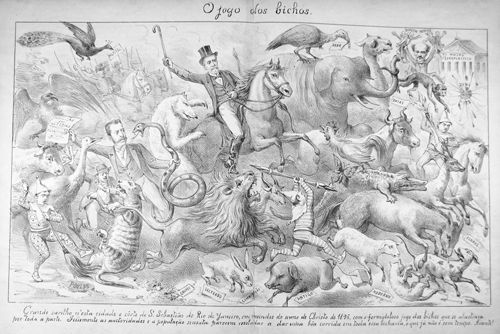
\includegraphics[width=\textwidth, height=6cm]{images/bicho01.jpg}
 \end{minipage}
 \hfill
 \begin{minipage}[b]{0.45\textwidth}
  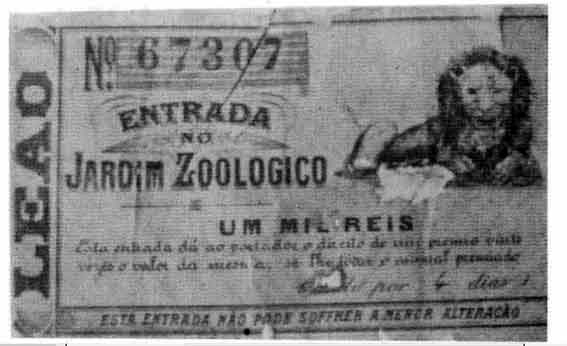
\includegraphics[width=\textwidth, height=6cm]{images/bicho02.jpg}
 \end{minipage}
 \caption{Left: cartoon of the Baron of Drummond and the animals of the \emph{jogo do bicho} (1896). Right: entry ticket to Rio's Zoological Garden that allowed the bearer to join the raffle. Sources: Instituto Histórico e Geográfico Brasileiro, Rio de Janeiro, Revista Illustrada, ano 21, no. 718 (1896) and Museu da Imagem e do Som, Rio de Janeiro. Reproduced in \citet[35--36]{chazkel2011laws}.}
 \label{fig:barao}
\end{figure}

Vivamus pulvinar elit dolor, eu rhoncus risus vulputate eu. Nunc in nulla id lacus blandit semper. Vivamus at porttitor diam, quis malesuada diam. Suspendisse efficitur molestie maximus. Maecenas accumsan cursus magna pellentesque sollicitudin. Vivamus bibendum commodo auctor. Nulla luctus efficitur quam in mattis. Curabitur pharetra, ligula id placerat fermentum, velit est vestibulum mauris, a malesuada neque mi a arcu. Sed ac pulvinar arcu. Sed ligula sem, consectetur id risus nec, condimentum posuere augue. Morbi faucibus, est vel finibus sollicitudin, elit ligula dapibus orci, sed fermentum velit eros non ex. Nunc dolor quam, consequat sit amet lacinia sit amet, eleifend efficitur.

Curabitur pellentesque gravida erat, eleifend lobortis arcu pharetra sit amet. Nunc tincidunt varius tortor vel viverra. Suspendisse sollicitudin gravida magna, id rhoncus risus volutpat a. Quisque ac luctus sem, sagittis cursus neque. Suspendisse pretium leo volutpat tortor consequat, ut placerat metus tincidunt. Morbi eleifend placerat vulputate. Praesent ornare, lacus at fermentum interdum, enim arcu pretium risus, vel molestie purus elit volutpat sapien. In euismod quam non nunc aliquet finibus. Donec vulputate hendrerit est quis porttitor. Cras a diam rutrum, vehicula urna quis, congue mi. Aliquam libero quam, molestie nec nisi nec, sollicitudin finibus nibh.

Pellentesque maximus vehicula egestas. In aliquam sagittis odio, non mattis felis. Ut gravida tortor venenatis, venenatis odio quis, ultricies lorem. Aliquam tristique eros lacinia enim posuere bibendum. Sed ac arcu at tortor rutrum ultricies. Aenean accumsan, massa sit amet viverra pulvinar, purus orci tristique augue, sit amet commodo tellus sem ac nibh. 

\begin{figure}[!htbp]
 \centering
 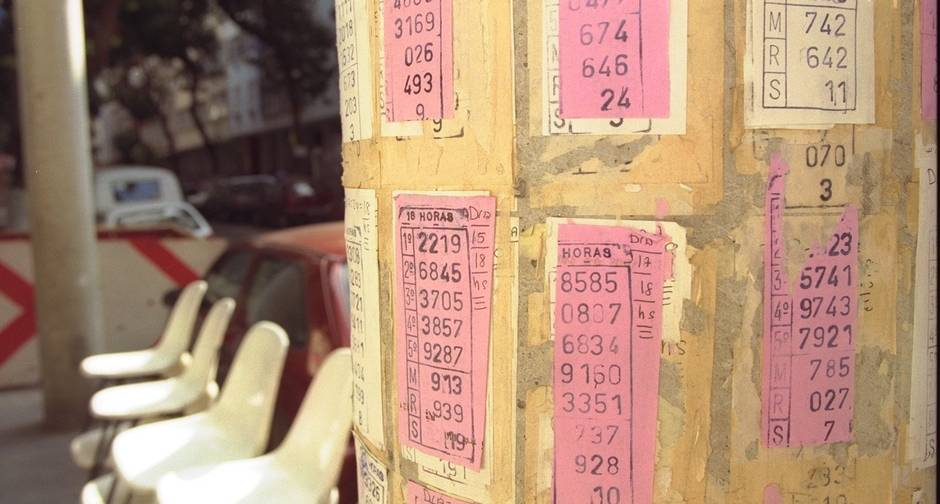
\includegraphics[width=\textwidth, height=6cm]{images/bicho05.jpg}
 \caption{\emph{Jogo do bicho} results are fixed on light poles in Rio de Janeiro. Source: \citet{gomes1998bicho}.}
 \label{fig:poste}
\end{figure}

\begin{align}
 f(x)  &= a x^2+b x +c   &   g(x)  &= d x^3 \\
 f'(x) &= 2 a x +b       &   g'(x) &= 3 d x^2
\end{align}


\begin{equation}
  u(x) = 
  \begin{cases} 
   \exp{x} & \text{if } x \geq 0 \\
   1       & \text{if } x < 0
  \end{cases}
\end{equation}

% Table

\def\onepc{$^{\ast\ast}$} \def\fivepc{$^{\ast}$}
\def\tenpc{$^{\dag}$}
\def\legend{\multicolumn{4}{l}{\footnotesize{Significance levels
:\hspace{1em} $\dag$ : .1 \hspace{1em}
$\ast$ : .05 \hspace{1em} $\ast\ast$ : .01 \normalsize}}}

\begin{table}[htbp]\centering \footnotesize \caption{Logistic Regressions for Civil War Incidence \label{table1:sumstats}}
\begin{tabular}{l c c c}\hline\hline
\multicolumn{1}{c}{\textbf{Variable}} & \textbf{Model I}
 & \textbf{Model II}& \textbf{Model III}\\ \hline
p\_xrcomp1$_{t-1}$ & $-$0.914**\\
(selection) & (0.184)\\
p\_xrcomp2$_{t-1}$ & $-$2.218**\\
(dual / transition) & (0.391)\\
p\_xrcomp3$_{t-1}$ & $-$0.783**\\
(election) & (0.236)\\
p\_xrcomp\_n$_{t-1}$ & 0.457\\
(autocratisation) & (0.440)\\
p\_xrcomp\_p$_{t-1}$ & 0.150\\
(democratisation) & (0.430)\\
dpi\_eipc3$_{t-1}$ & & $-$0.091*\\
(election, 1 candidate) & & (0.178)\\
dpi\_eipc4$_{t-1}$ & & $-$2.203*\\
(1 party elec., many candidates) & & (1.065)\\
dpi\_eipc6$_{t-1}$  & & $-$0.549$\dagger$\\
(multiparty elec., winner > 75\%) & & (0.304)\\
dpi\_eipc7$_{t-1}$ & & $-$0.202\\
(multiparty elec., winner < 75\%) & & (0.183)\\
dpi\_eipc\_n$_{t-1}$ & & 0.710$\dagger$\\
(autocratisation) & & (0.387)\\
dpi\_eipc\_p$_{t-1}$ & & 0.431\\
(democratisation) & & (0.297)\\
van\_comp$_{t-1}$ & & & $-$.008**\\
(\% winning party) & & & (0.003)\\
no\_ufs$_{t-1}$ & 0.780** & 0.784** & 0.747**\\
(unitarian) & (0.194) & (0.187) & (0.175)\\
r\_atlas & 1.141** & 1.157** & 1.308**\\
(eth. frac.) & (0.256) & (0.255) & (0.241)\\
oil$_{t-1}$ & 0.249 & 0.248 & 0.234\\
(> 1/3 oil exp.) & (0.176) & (0.175) & (0.160)\\
lmtnest & 0.331** & 0.324** & 0.333**\\
(ln mount. terrain) & (0.050) & (0.045) & (0.043)\\
ln\_unna\_pop$_{t-1}$ & 0.331** & 0.240** & 0.265**\\
(ln population) & (0.048) & (0.046) & (0.043)\\
unna\_grgdp$_{t-1}$ & $-$0.028* & $-$0.029** & $-$0.025**\\
(gdp growth) & (0.011) & (0.009) & (0.009)\\
ln\_gdpc$_{t-1}$ & $-$0.144* & $-$0.186** & $-$0.131**\\
(ln gdp per cap.) & (0.064) & (0.062) & (0.446)\\
constant & $-$7.599** & $-$6.357** & $-$7.136**\\
\hline
N & 2579 & 2600 & 2819\\
Wald $\chi^2$ & (8) 174.63 & (13) 154.40 & (8) 174.63\\
Log Pseudolikelihood & $-$779.945 & $-$844.045 & $-$916.790\\
Pseudo R$^2$ & 0.115 & 0.100 & 0.102\\
\hline
\legend\\
{\footnotesize Standard errors in parentheses}\\
\hline
\end{tabular}
\end{table}